\section{Exercise one}

Consider the stochastic process defined by the following diagram:
\begin{figure}[H]
    \centering
    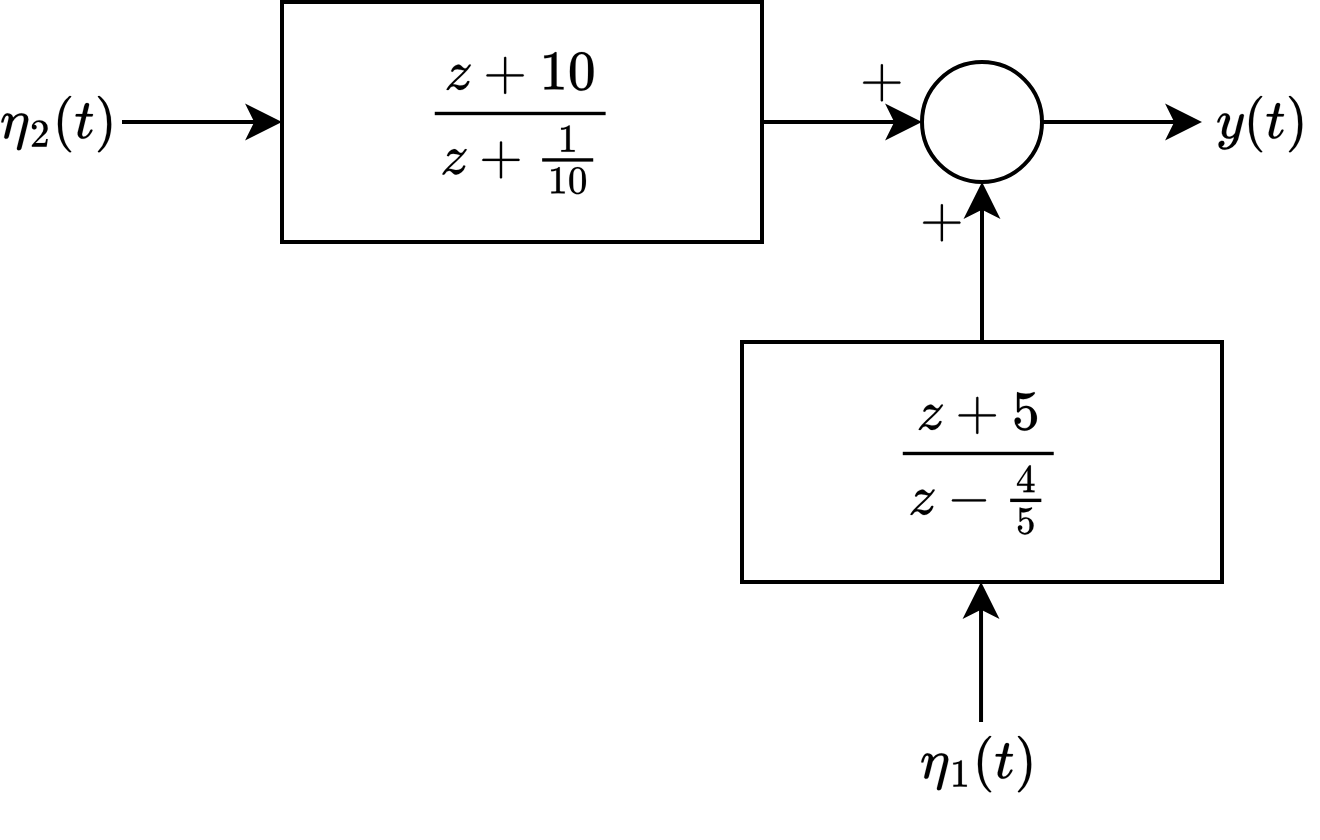
\includegraphics[width=0.5\linewidth]{images/block.png}
\end{figure}
Here, $\eta_1 \sim WN(1,1)$ and $\eta_2 \sim WN(0,1)$ are uncorrelated. 

Find the characteristic values of the given process $y(t)$.

\subsection*{Solution}
Remember that for an ARMA($n_a,n_b$) process:
\begin{itemize}
    \item If $n_a>n_b$, the covariance becomes recursive for $\tau=n_a$.
    \item If $n_a \leq n_b$, the covariance becomes recursive for $\tau=n_b+1$
\end{itemize}

The output process is composed of two uncorrelated processes because the  White Noise sources are uncorrelated:
\[y(t)=y_1(t)+y_2(t)\]
Since both $y_1(t)$ and $y_2(t)$ are stationary, $y(t)$ is also stationary.

The mean is: 
\[m_y=\mathbb{E}\left[y(t)\right]=\mathbb{E}\left[y_1(t)+y_2(t)\right]=W_1(1)\mathbb{E}\left[\eta_1(t)\right]+W_2(1)\mathbb{E}\left[\eta_2(t)\right]=\dfrac{15}{2}\]

The covariance can be computed as the sum of the covariances of $y_1(t)$ and $y_2(t)$ (since they are uncorrelated):
\[\gamma_y(\tau)=\gamma_{y_1}(\tau)+\gamma_{y_2}(\tau)\]

For the stochastic process $y_1(t)$ in the time domain:
\[y_1(t)=\dfrac{1}{5}y_1(t-1)+\eta_1(t)+5\eta_1(t-1)\]
Define the unbiased process by:
\[\begin{cases}
    \tilde{y}_1(t)=y_1(t)-m_{y_1}\\
    \tilde{\eta}_1(t)=\eta_1(t)-m_{\eta_1}
\end{cases}\]
Then, the process becomes:
\[\tilde{y}_1(t)=\dfrac{1}{5}\tilde{y}_1(t-1)+\tilde{\eta}_1(t)+5\tilde{\eta}_1(t-1)\]
The covariance at different time lags is:
\[\gamma_{y_1}(\tau)=\begin{cases}
    \frac{175}{6} \qquad\qquad\qquad\qquad \tau=0 \\
    \frac{65}{6} \qquad\qquad\qquad\qquad \left\lvert \tau\right\rvert =1 \\
    \frac{13}{6} \qquad\qquad\qquad\qquad \left\lvert \tau\right\rvert =2 \\
    \frac{1}{5}\gamma_{y_1}(\tau-1) \qquad\qquad \left\lvert \tau\right\rvert \geq 3 
\end{cases}\]

For the stochastic process $y_2(t)$:
\[y_2(t)=-\dfrac{1}{10}y_2(t-1)+\eta_2(t)+10\eta_2(t-1)\]
The covariance function is:
\[\gamma_{y_2}(\tau)=\begin{cases}
    100 \qquad\: \tau=0 \\
    0 \qquad\quad  \left\lvert \tau\right\rvert \geq 1
\end{cases}\]